\pdfoutput=1
\documentclass[preview]{standalone}

\usepackage[scale=0.7, vmarginratio=1:1]{geometry} 

\usepackage[utf8]{inputenc}
\usepackage{lmodern}
\usepackage[T1]{fontenc}

\usepackage{verbatim}
\usepackage{graphicx}
	\DeclareGraphicsRule{*}{mps}{*}{}
\usepackage{xcolor}

\usepackage{tikz}
	\usetikzlibrary{calc}
	\usetikzlibrary{arrows}
	\usetikzlibrary{backgrounds}
	\usetikzlibrary{decorations.pathmorphing}
	\usetikzlibrary{shapes.geometric}
	\tikzset{>=latex'}

\usepackage{amsmath}
\usepackage{amssymb}
\usepackage{dsfont}
\usepackage{nicefrac}
\usepackage{mathrsfs}
\usepackage[Euler]{upgreek}
\usepackage[nointegrals]{wasysym}
\usepackage{booktabs}
\usepackage{float}

\begin{document}

\centering

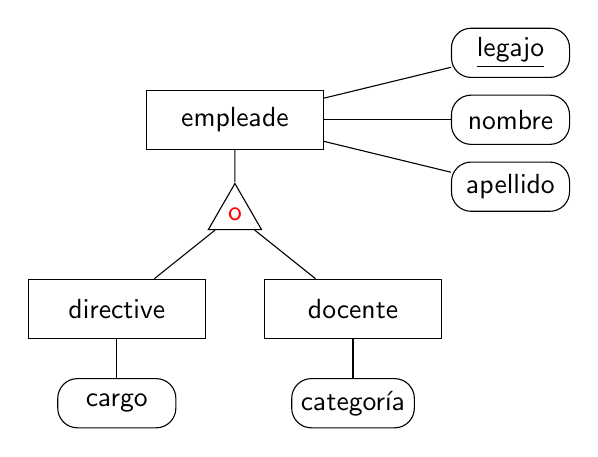
\begin{tikzpicture}[font=\sffamily]
	\node[draw,minimum width=2.25cm,minimum height=0.75cm] (empleade) at (0,0) {empleade};
	\node[draw,rounded corners=2.5mm,minimum width=1.5cm,minimum height=6.25mm] (legajo) at (3.5,0.85) {$\underline{\text{legajo}}$};
	\node[draw,rounded corners=2.5mm,minimum width=1.5cm,minimum height=6.25mm] (nombre) at (3.5,0.0) {nombre};
	\node[draw,rounded corners=2.5mm,minimum width=1.5cm,minimum height=6.25mm] (apellido) at (3.5,-0.85) {apellido};
	\draw (empleade)--(legajo);
	\draw (empleade)--(nombre);
	\draw (empleade)--(apellido);
	\node[draw,regular polygon,regular polygon sides=3,inner sep=0.5mm] (herencia) at (0,-1.2) {\textcolor{red}{o}};
	\node[draw,minimum width=2.25cm,minimum height=0.75cm] (directive) at (-1.5,-2.4) {directive};
	\node[draw,rounded corners=2.5mm,minimum width=1.5cm,minimum height=6.25mm] (attr1) at (-1.5,-3.6) {cargo};
	\node[draw,minimum width=2.25cm,minimum height=0.75cm] (docente) at (1.5,-2.4) {docente};
	\node[draw,rounded corners=2.5mm,minimum width=1.5cm,minimum height=6.25mm] (attr2) at (1.5,-3.6) {categoría};
	\draw (directive)--(attr1) (docente)--(attr2);
	\draw (empleade)--(herencia)--(directive) (herencia)--(docente);
\end{tikzpicture}

\vskip 12pt

\sffamily
{\large empleade(\underline{legajo}, nombre, apellido, cargo, categoría)}
\textcolor{red}{\scriptsize $\leftarrow$ sin tipo}

\end{document}
